\documentclass[11pt,letterpaper]{article}
\usepackage[lmargin=2.2in,rmargin=0.7in,tmargin=1.0in,bmargin=1.0in]{geometry}
\usepackage{notes}

\begin{document}

\begin{center}
\Large\textbf{DAY 40 -- Nonlinear Mechanics: The Pendulum}\\
\normalsize Section 5.2
\end{center}

%%%%%%%%%%%%%%%%%%%%%%%%%%%%%%%%%%%%%%%%%%%%%%%%%%%%%%%%%%%%%%%%%%%%%%%%
\section{The Pendulum Equation}

\subsection{Setup and Sign Convention}

A pendulum consists of a bob of mass $m$ attached
to a pivot by a weightless rigid rod of length $L$.
The rod can rotate in a vertical plane.

Let $\theta(t)$ be the angle measured from the
downward vertical. We take counterclockwise rotation
to be positive. Near the hanging position:
\begin{itemize}
    \item $\theta>0$ places the bob to the right;
    \item $\theta<0$ places the bob to the left.
\end{itemize}

The initial conditions are
\[
\theta(0)=\theta_0,
\qquad
\theta'(0)=v_0,
\]
where $v_0$ is the initial angular velocity.

\begin{center}
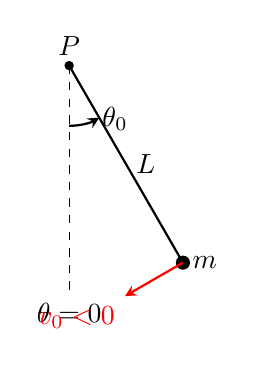
\begin{tikzpicture}[scale=0.85,>=stealth]
    \def\pendL{3.4}
    \def\pendAngle{30}

    \coordinate (P) at (0,0);
    \coordinate (M) at
        ({\pendL*sin(\pendAngle)},
         {-\pendL*cos(\pendAngle)});

    \draw[dashed] (P)--(0,-\pendL)
        node[below] {$\theta=0$};
    \draw[thick] (P)--(M)
        node[midway,right] {$L$};

    \fill (P) circle (2pt) node[above] {$P$};
    \fill (M) circle (3pt) node[right] {$m$};

    \draw[->,thick] (0,-0.9)
        arc[start angle=-90,
            end angle={-90+\pendAngle},radius=0.9];
    \node[right] at (0.35,-0.8) {$\theta_0$};

    \draw[red,thick,->] (M)
        --++({-cos(\pendAngle)},{-sin(\pendAngle)})
        node[below left] {$v_0<0$};
\end{tikzpicture}
\end{center}

The diagram shows a positive initial angle and
a negative initial angular velocity.

Our goal is to derive an equation for $\theta(t)$.

%-------------------------------------------------------------
\subsection{Forces on the Bob}

There are three contributions:
\begin{itemize}
    \item Gravity acts vertically downward.
    \item The rod exerts a force along its length.
    \item Resistance opposes the motion.
\end{itemize}

The rod force has no tangential component.
The signed tangential component of gravity is
\[
F_{\mathrm{gravity},t}=-mg\sin\theta.
\]
The negative sign makes gravity pull the pendulum
toward the hanging position.

We model resistance as proportional to tangential
velocity. Since that velocity is $L\theta'$,
\[
F_d=-bL\theta',
\qquad b\ge0.
\]

\begin{figure}[H]
\centering
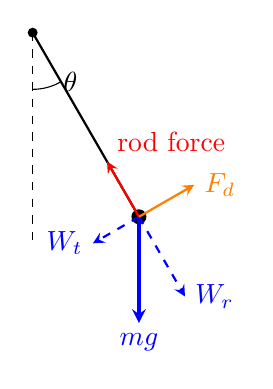
\begin{tikzpicture}[scale=0.9,>=stealth]
    \def\pendL{3}
    \def\pendAngle{30}
    \def\weightLength{1.5}

    \coordinate (P) at (0,0);
    \coordinate (M) at
        ({\pendL*sin(\pendAngle)},
         {-\pendL*cos(\pendAngle)});

    \draw[dashed] (P)--(0,-\pendL);
    \draw[thick] (P)--(M);
    \fill (P) circle (2pt);
    \fill (M) circle (3pt);

    \draw (0,-0.8)
        arc[start angle=-90,
            end angle={-90+\pendAngle},radius=0.8];
    \node[right] at (0.3,-0.7) {$\theta$};

    % Weight
    \draw[blue,very thick,->]
        (M)--++(0,-\weightLength)
        node[below] {$mg$};

    % Radial component of weight
    \draw[blue,dashed,thick,->]
        (M)--++
        ({\weightLength*cos(\pendAngle)*sin(\pendAngle)},
         {-\weightLength*cos(\pendAngle)*cos(\pendAngle)})
        node[right] {$W_r$};

    % Tangential component of weight
    \draw[blue,dashed,thick,->]
        (M)--++
        ({-\weightLength*sin(\pendAngle)*cos(\pendAngle)},
         {-\weightLength*sin(\pendAngle)*sin(\pendAngle)})
        node[left] {$W_t$};

    % Rod force, shown inward for this configuration
    \draw[red,thick,->] (M)--++
        ({-0.9*sin(\pendAngle)},{0.9*cos(\pendAngle)})
        node[above right] {rod force};

    % Resistance for leftward motion
    \draw[orange,thick,->] (M)--++
        ({0.9*cos(\pendAngle)},{0.9*sin(\pendAngle)})
        node[right] {$F_d$};
\end{tikzpicture}
\caption{Forces when the bob is moving to the left.
Resistance points opposite the velocity.
The dashed arrows show the components of gravity.}
\end{figure}

Although the rod has fixed length, the radial forces
do not generally cancel: their resultant provides
centripetal acceleration. To find $\theta(t)$,
we use the tangential equation.

%-------------------------------------------------------------
\subsection{Newton's Second Law}

The signed arc length is $s=L\theta$, so the
tangential acceleration is
\[
s''=L\theta''.
\]
Newton's second law in the tangential direction gives
\begin{align*}
\sum F_t&=mL\theta'',\\
-mg\sin\theta-bL\theta'&=mL\theta''.
\end{align*}
Rearranging,
\[
mL\theta''+bL\theta'+mg\sin\theta=0.
\]
Divide by $mL$ and define
\[
\gamma=\frac{b}{m},
\qquad
\omega=\sqrt{\frac{g}{L}}.
\]
Then
\[
\boxed{
\theta''+\gamma\theta'+\omega^2\sin\theta=0.
}
\]
This is the \textbf{damped pendulum equation}.
It is nonlinear because of $\sin\theta$.

%-------------------------------------------------------------
\subsection{Connection to the Spring Equation}

For small angles measured in radians,
\[
\sin\theta\approx\theta.
\]
The pendulum equation then becomes
\[
\theta''+\gamma\theta'+\omega^2\theta=0.
\]
This has the same form as the spring equation.

The parameter $\omega=\sqrt{g/L}$ is the
\textbf{small-angle natural angular frequency}.
For large swings, the period depends on amplitude.

%%%%%%%%%%%%%%%%%%%%%%%%%%%%%%%%%%%%%%%%%%%%%%%%%%%%%%%%%%%%%%%%%%%%%%%%
\section{The Pendulum without Friction}

\subsection{Rewriting as a System}

Set $\gamma=0$ and choose $\omega^2=4$:
\[
\theta''+4\sin\theta=0.
\]
Introduce
\[
x=\theta,\qquad y=\theta'.
\]
Then
\[
\boxed{
\theta''+4\sin\theta=0
\quad\Longleftrightarrow\quad
\begin{dcases}
x'=y,\\
y'=-4\sin x.
\end{dcases}
}
\]
This is a first-order \textbf{nonlinear} system.

The horizontal coordinate records angle; the vertical
coordinate records angular velocity.

%-------------------------------------------------------------
\subsection{Equilibria and Linearization}

\begin{example}[1]{
Find the equilibria and analyze their linearizations:
\[
\begin{dcases}
x'=y,\\
y'=-4\sin x.
\end{dcases}
\]
}

\paragraph{Step 1. Find the equilibria.}
Set both derivatives equal to zero:
\[
y=0,\qquad \sin x=0.
\]
Therefore,
\[
\boxed{(n\pi,0),\qquad n\in\mathbb Z.}
\]
There are infinitely many equilibrium points
in the unwrapped angle coordinate.

\paragraph{Step 2. Compute the Jacobian.}
The Jacobian is
\[
\boxed{
J(x,y)=
\begin{pmatrix}
0&1\\
-4\cos x&0
\end{pmatrix}.
}
\]
At an equilibrium,
\[
\cos(n\pi)=(-1)^n,
\]
so we consider even and odd multiples separately.

\paragraph{Step 3. Analyze the even multiples.}
At $(2n\pi,0)$,
\[
J=
\begin{pmatrix}
0&1\\
-4&0
\end{pmatrix}.
\]
The characteristic equation is
\[
\lambda^2+4=0,
\qquad \lambda=\pm2i.
\]
The linearized system has a center.

In coordinates $u=x-2n\pi$ and $v=y$,
\[
u'=v,\qquad v'=-4u.
\]
Its trajectories satisfy
\[
4u^2+v^2=C,
\]
so they are vertically stretched ellipses.
At $(u,v)=(1,0)$ the velocity is $(0,-4)$,
giving clockwise motion.

Purely imaginary eigenvalues alone do not establish
a nonlinear center. We will confirm the centers
using energy conservation.

\paragraph{Step 4. Analyze the odd multiples.}
At $((2n+1)\pi,0)$,
\[
J=
\begin{pmatrix}
0&1\\
4&0
\end{pmatrix}.
\]
The characteristic equation is
\[
\lambda^2-4=0,
\qquad \lambda=\pm2.
\]
Thus,
\[
\boxed{\text{Every odd-multiple equilibrium is a saddle}.}
\]

Corresponding eigenvectors are
\[
\lambda_u=2:
\quad
\mathbf{v}_u=\begin{pmatrix}1\\2\end{pmatrix},
\qquad
\lambda_s=-2:
\quad
\mathbf{v}_s=\begin{pmatrix}1\\-2\end{pmatrix}.
\]
The unstable tangent direction has slope $2$,
and the stable tangent direction has slope $-2$.
\end{example}

%-------------------------------------------------------------
\subsection{Physical Meaning of the Equilibria}

At an equilibrium, the angular velocity is zero.

\begin{itemize}
    \item $x=2n\pi$: the bob hangs straight down.
    \item $x=(2n+1)\pi$: the bob stands straight up.
\end{itemize}

Angles differing by $2\pi$ represent the same physical
orientation. Keeping $x$ unwrapped lets us track
complete revolutions.

%%%%%%%%%%%%%%%%%%%%%%%%%%%%%%%%%%%%%%%%%%%%%%%%%%%%%%%%%%%%%%%%%%%%%%%%
\section{Energy and the Undamped Phase Portrait}

\subsection{Conservation of Energy}

Multiply
\[
\theta''+\omega^2\sin\theta=0
\]
by $\theta'$:
\[
\theta'\theta''+\omega^2\theta'\sin\theta=0.
\]
Recognizing derivatives,
\[
\frac{d}{dt}
\left[
\frac12(\theta')^2+\omega^2(1-\cos\theta)
\right]=0.
\]
Therefore,
\[
\boxed{
E(x,y)=\frac12y^2+\omega^2(1-\cos x)
=\text{constant}.
}
\]
This is the mechanical energy divided by $mL^2$.
The first term represents kinetic energy and the
second represents gravitational potential energy.

For our equation with $\omega^2=4$,
\[
\boxed{E(x,y)=\frac12y^2+4(1-\cos x).}
\]

%-------------------------------------------------------------
\subsection{Energy Levels and Trajectories}

Each trajectory lies on an energy level curve.

At a downward equilibrium,
\[
E(2n\pi,0)=0.
\]
At an upright equilibrium,
\[
E((2n+1)\pi,0)=8.
\]
Thus, $E=8$ is the energy needed to reach the
upright position with zero speed.

The energy levels give three types of nonconstant motion:
\begin{itemize}
    \item \textbf{$0<E<8$: oscillation.}
    Closed curves surround a downward equilibrium.
    The pendulum swings back and forth.

    \item \textbf{$E=8$: separatrix motion.}
    The pendulum approaches an upright equilibrium
    asymptotically.

    \item \textbf{$E>8$: rotation.}
    The angular velocity never reaches zero,
    so the pendulum continues rotating.
\end{itemize}

The closed energy curves confirm that the downward
equilibria are centers. They are stable but not
asymptotically stable.

%-------------------------------------------------------------
\subsection{The Phase Portrait}

Near the centers, the closed curves resemble the
ellipses predicted by linearization. Larger curves
are not exact ellipses.

The curves at $E=8$ are called \textbf{separatrices}
because they separate oscillations from rotations.
They satisfy
\[
\frac12y^2+4(1-\cos x)=8,
\]
or
\[
y=\pm4\left|\cos\frac{x}{2}\right|.
\]

\begin{center}
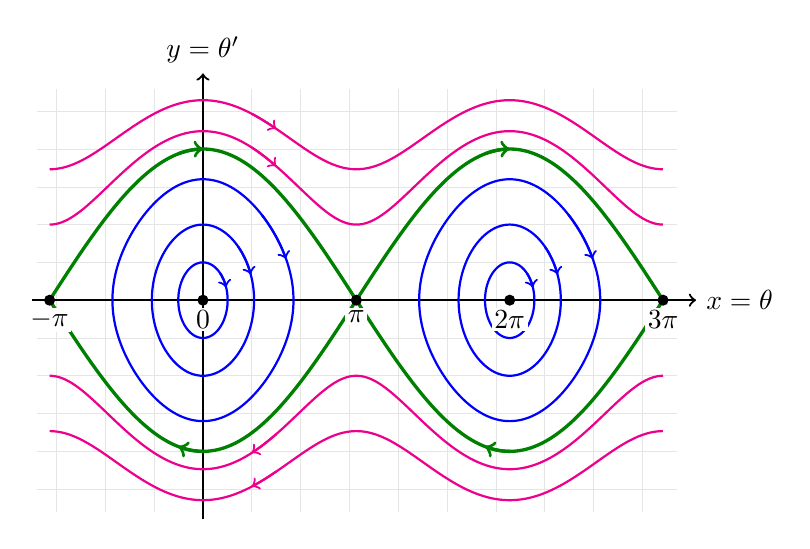
\begin{tikzpicture}[x=0.62cm,y=0.48cm]
    \draw[step=1,very thin,gray!20]
        (-3.4,-5.6) grid (9.7,5.6);

    \draw[->,thick] (-3.5,0)--(10.1,0)
        node[right] {$x=\theta$};
    \draw[->,thick] (0,-5.8)--(0,6)
        node[above] {$y=\theta'$};

    % Exact closed energy curves.
    % Parameterization:
    % x = center + 2 asin(k sin q), y = 4k cos q.
    % The plotting parameter q is not physical time.
    \foreach \center in {0,6.283185}{
        \foreach \k in {0.25,0.5,0.8}{
            \draw[blue,thick,domain=0:360,samples=220]
                plot
                ({\center+2*rad(asin(\k*sin(\x)))},
                 {4*\k*cos(\x)});

            \draw[blue,thick,->,domain=45:70,samples=25]
                plot
                ({\center+2*rad(asin(\k*sin(\x)))},
                 {4*\k*cos(\x)});
        }
    }

    % Separatrices
    \foreach \center in {0,6.283185}{
        \draw[green!50!black,very thick,
              domain=-pi:pi,samples=180]
            plot ({\center+\x},{4*cos(deg(\x/2))});
        \draw[green!50!black,very thick,
              domain=-pi:pi,samples=180]
            plot ({\center+\x},{-4*cos(deg(\x/2))});

        \draw[green!50!black,very thick,->,
              domain=-0.5:0,samples=20]
            plot ({\center+\x},{4*cos(deg(\x/2))});
        \draw[green!50!black,very thick,->,
              domain=0:-0.5,samples=20]
            plot ({\center+\x},{-4*cos(deg(\x/2))});
    }

    % Rotational energy curves
    \foreach \energy in {10,14}{
        \draw[magenta,thick,domain=-pi:3*pi,samples=300]
            plot
            (\x,{sqrt(2*\energy-8*(1-cos(deg(\x))))});
        \draw[magenta,thick,domain=-pi:3*pi,samples=300]
            plot
            (\x,{-sqrt(2*\energy-8*(1-cos(deg(\x))))});

        \draw[magenta,thick,->,domain=1:1.5,samples=20]
            plot
            (\x,{sqrt(2*\energy-8*(1-cos(deg(\x))))});
        \draw[magenta,thick,->,domain=1.5:1,samples=20]
            plot
            (\x,{-sqrt(2*\energy-8*(1-cos(deg(\x))))});
    }

    % Equilibria and labels
    \foreach \n/\label in {-1/{-\pi},0/0,1/\pi,2/{2\pi},3/{3\pi}}{
        \fill ({pi*\n},0) circle (2pt);
        \node[below,fill=white,inner sep=1pt]
            at ({pi*\n},-0.18) {$\label$};
    }
\end{tikzpicture}

\small
Blue: oscillations.
Green: separatrices.
Magenta: rotations.
\end{center}

Above the $x$-axis, $x'=y>0$, so trajectories move
to the right. Below it, they move to the left.

%-------------------------------------------------------------
\subsection{Three Initial Velocities}

\begin{example}[2]{
For
\[
\theta''+4\sin\theta=0,\qquad \theta(0)=0,
\]
describe the motion for each initial angular velocity:
\[
\text{(a) }\theta'(0)=2,\qquad
\text{(b) }\theta'(0)=5,\qquad
\text{(c) }\theta'(0)=4.
\]
}

\paragraph{Step 1. Find the initial energy.}
Since $\theta(0)=0$,
\[
E=\frac12\bigl(\theta'(0)\bigr)^2.
\]
Compare this value with the separatrix energy $8$.

\paragraph{Step 2. Classify each motion.}

\textbf{(a) Initial velocity $2$.}
\[
E=\frac12(2)^2=2<8.
\]
The pendulum swings back and forth indefinitely.
At a turning point, $\theta'=0$, so
\[
4(1-\cos\theta)=2
\implies \cos\theta=\frac12.
\]
Thus, the turning angles are $\theta=\pm\pi/3$.

\medskip
\textbf{(b) Initial velocity $5$.}
\[
E=\frac12(5)^2=\frac{25}{2}>8.
\]
The pendulum has enough energy to rotate over
the top repeatedly. Its angular velocity remains positive.

\medskip
\textbf{(c) Initial velocity $4$.}
\[
E=\frac12(4)^2=8.
\]
The solution follows a separatrix:
\[
\theta(t)\to\pi,
\qquad
\theta'(t)\to0
\quad\text{as }t\to\infty.
\]
It approaches the upright position but does not
reach it in finite time.
\end{example}

\begin{figure}[H]
    \centering
    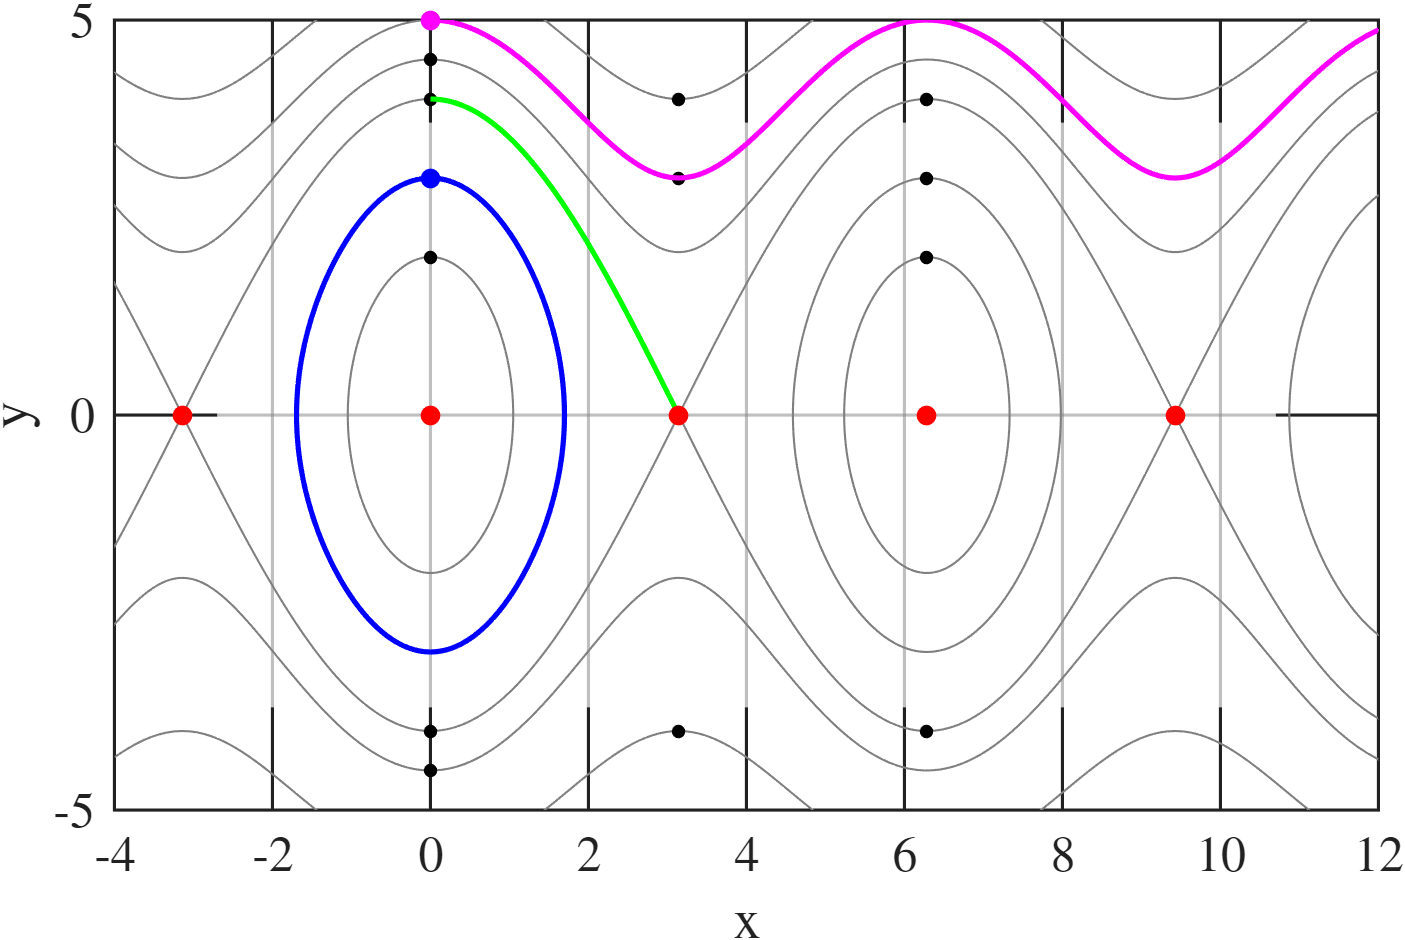
\includegraphics[width=0.9\linewidth]
        {figs/pend_phase1.png}
    \caption{Trajectories for the three initial velocities.
    Blue: oscillation. Magenta: rotation.
    Green: asymptotic approach to the upright equilibrium.}
\end{figure}

%%%%%%%%%%%%%%%%%%%%%%%%%%%%%%%%%%%%%%%%%%%%%%%%%%%%%%%%%%%%%%%%%%%%%%%%
\section{The Pendulum with Friction}

\subsection{The Damped System}

With positive damping,
\[
\theta''+\gamma\theta'+\omega^2\sin\theta=0,
\qquad \gamma,\omega>0.
\]
Using $x=\theta$ and $y=\theta'$ gives
\[
\boxed{
\begin{dcases}
x'=y,\\
y'=-\gamma y-\omega^2\sin x.
\end{dcases}
}
\]
The equilibria remain
\[
\boxed{(n\pi,0),\qquad n\in\mathbb Z.}
\]
Damping changes their stability and the surrounding
trajectories.

%-------------------------------------------------------------
\subsection{Energy Loss}

Use the same energy function:
\[
E(x,y)=\frac12y^2+\omega^2(1-\cos x).
\]
Along a damped solution,
\begin{align*}
\frac{dE}{dt}
&=yy'+\omega^2\sin x\,x'\\
&=y(-\gamma y-\omega^2\sin x)
+\omega^2\sin x\,y\\
&=-\gamma y^2.
\end{align*}
Therefore,
\[
\boxed{\frac{dE}{dt}=-\gamma y^2\le0.}
\]
Energy decreases whenever the bob is moving.
Consequently, nonconstant closed trajectories
are no longer possible.

%-------------------------------------------------------------
\subsection{Classifying the Equilibria}

\begin{example}[3]{
Classify the equilibria of the damped pendulum:
\[
\begin{dcases}
x'=y,\\
y'=-\gamma y-\omega^2\sin x,
\end{dcases}
\qquad \gamma,\omega>0.
\]
}

\paragraph{Step 1. Compute the Jacobian.}
The Jacobian is
\[
J(x,y)=
\begin{pmatrix}
0&1\\
-\omega^2\cos x&-\gamma
\end{pmatrix}.
\]

\paragraph{Step 2. Analyze the downward equilibria.}
At $(2n\pi,0)$,
\[
J=
\begin{pmatrix}
0&1\\
-\omega^2&-\gamma
\end{pmatrix}.
\]
The characteristic equation is
\[
\lambda^2+\gamma\lambda+\omega^2=0,
\]
so
\[
\lambda=
\frac{-\gamma\pm\sqrt{\gamma^2-4\omega^2}}{2}.
\]

There are three cases:
\begin{itemize}
    \item $0<\gamma<2\omega$:
    complex eigenvalues with negative real parts.
    The equilibrium is a \textbf{stable spiral}.

    \item $\gamma=2\omega$:
    the repeated eigenvalue is $\lambda=-\omega$.
    The linearized system has a
    \textbf{stable improper node}.

    \item $\gamma>2\omega$:
    two distinct negative eigenvalues.
    The equilibrium is a \textbf{stable node}.
\end{itemize}
Every downward equilibrium is asymptotically stable.

\paragraph{Step 3. Analyze the upright equilibria.}
At $((2n+1)\pi,0)$,
\[
J=
\begin{pmatrix}
0&1\\
\omega^2&-\gamma
\end{pmatrix}.
\]
The characteristic equation is
\[
\lambda^2+\gamma\lambda-\omega^2=0.
\]
The product of the eigenvalues is $-\omega^2<0$,
so one is positive and the other is negative.

Therefore,
\[
\boxed{\text{Every upright equilibrium remains a saddle}.}
\]
\end{example}

%-------------------------------------------------------------
\subsection{Interpreting the Damping Cases}

The classifications describe motion near a downward
equilibrium:
\begin{itemize}
    \item \textbf{Underdamped}: the bob oscillates
    with decreasing amplitude.
    The phase portrait has a clockwise stable spiral.

    \item \textbf{Critically damped}: the bob approaches
    equilibrium without repeated oscillations.
    A crossing of equilibrium depends on the initial
    conditions; there is not necessarily one oscillation.

    \item \textbf{Overdamped}: the bob approaches
    equilibrium without repeated oscillations.
    The local phase portrait is a stable node.
\end{itemize}

Large initial velocities may produce complete rotations
before the pendulum settles. The node or spiral
classification describes its eventual local motion.

\begin{figure}[H]
\centering
\begin{subfigure}[t]{0.48\textwidth}
    \centering
    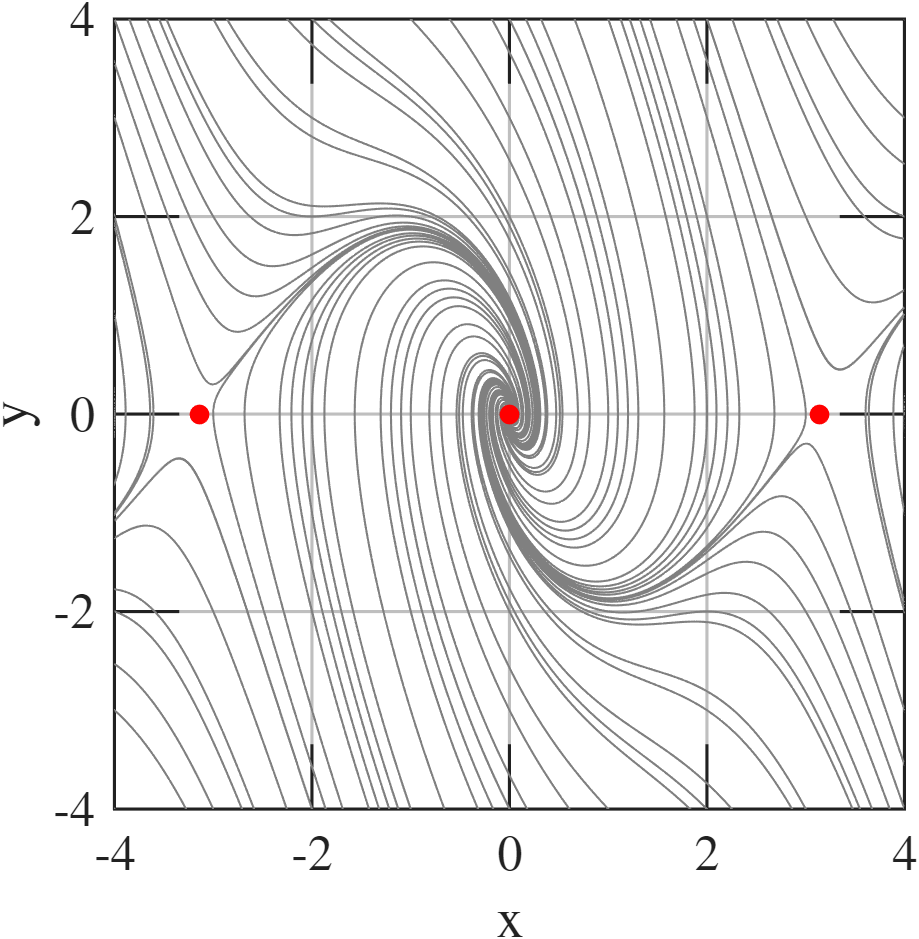
\includegraphics[width=\linewidth]
        {figs/pend_under.png}
    \caption{Underdamped: $0<\gamma<2\omega$.}
\end{subfigure}
\hfill
\begin{subfigure}[t]{0.48\textwidth}
    \centering
    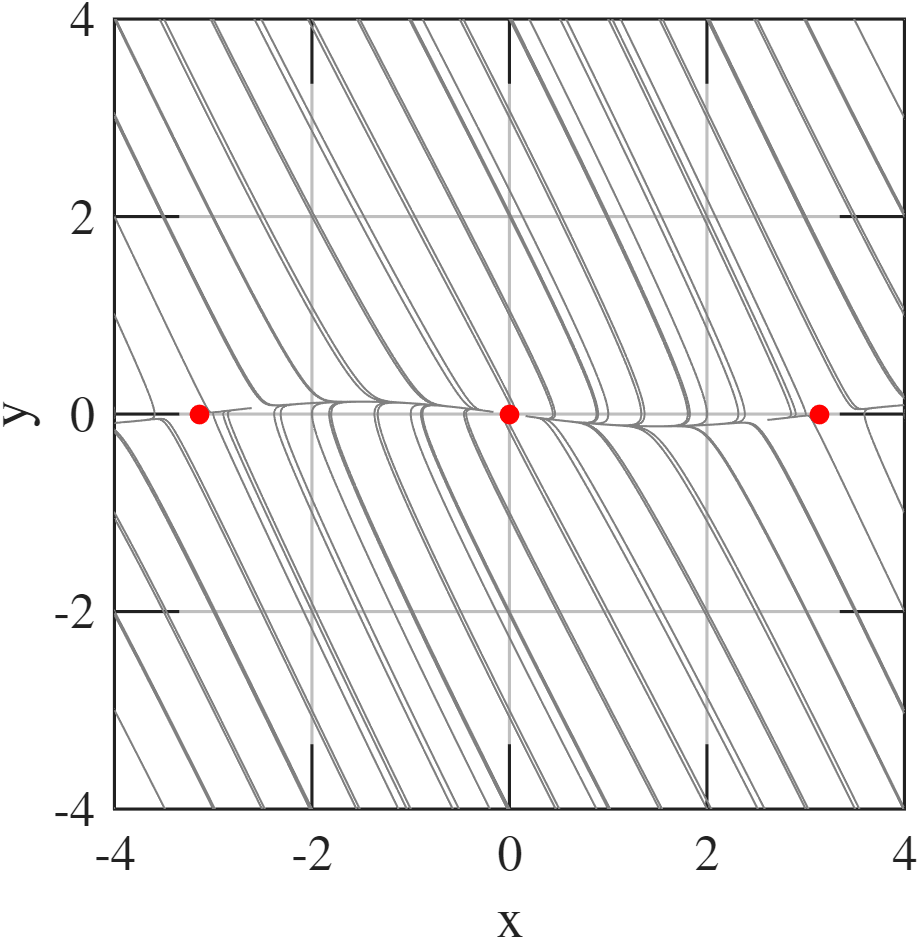
\includegraphics[width=\linewidth]
        {figs/pend_over.png}
    \caption{Overdamped: $\gamma>2\omega$.}
\end{subfigure}

\medskip

\begin{subfigure}[t]{0.48\textwidth}
    \centering
    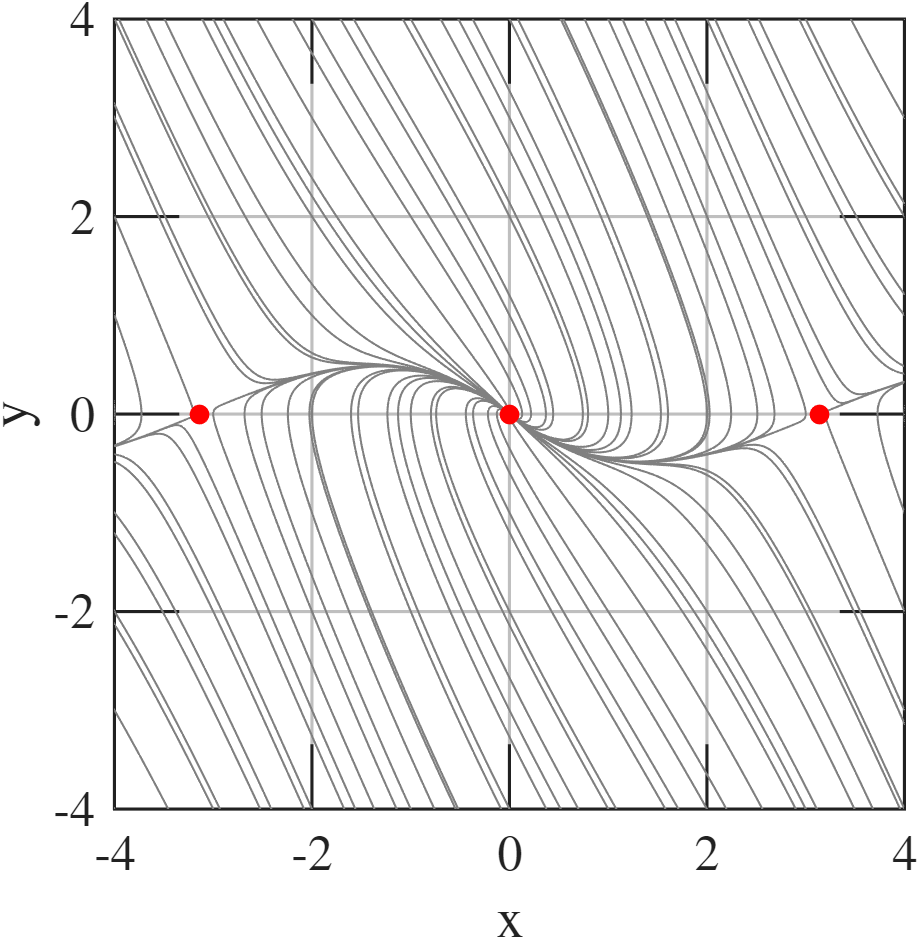
\includegraphics[width=\linewidth]
        {figs/pend_crit.png}
    \caption{Critically damped: $\gamma=2\omega$.}
\end{subfigure}

\caption{Damped pendulum phase portraits.
Downward equilibria are asymptotically stable;
upright equilibria remain saddles.}
\end{figure}

\end{document}